\section{Introduction}
\label{sec:intro}

Graph Neural Networks (GNNs) are %a type of 
neural network models computing functions over graphs or graph-node pairs. Their ability to extract feature and structural information from
%a given graph 
graphs
has made GNNs a promising candidate for% efficiently
tackling tasks in fields such as social network analysis, chemistry applications, and knowledge graphs. For a comprehensive survey of 
%general 
GNN applications, see \citet{ZhouCHZYLWLS20}, and for a survey of GNNs for knowledge graphs, see \citet{YeKSSW22}.

The increasing use of GNNs (or neural network-based models in general) leads to a heightened necessity for reliable safety guarantees or explanations of their behavior, in order to meet legal requirements or client desiderata. Let us illustrate some guarantees we may expect.

\begin{example}
\label{ex:gnn_social_network}
    Consider a GNN $N$ used to identify bots in a fictitious social network \texttt{NEWSNET} (see Figure~\ref{fig:gnn_social_network}). The network forms a graph where any registered account is a node and the edges represent relationships between accounts. In such a setting, the GNN decides, based on account-specific features, such as the frequency of posts or time of activity, whether an account is a regular human user or a (malicious) bot.

 For the trustworthiness of \texttt{NEWSNET}, it is essential that the GNN $N$  comes with guarantees such as:

    \begin{enumerate}
        \item[A\phantom{'}] ``Every account that spams $100$ messages or more per minute is identified as a bot by $N$.''
        \item[A'] ``If there is a significant, humanly impossible activity of a user within a short amount of time, then $N$ will identify it as a bot.''
        \item[B\phantom{'}] ``Every account whose friends send more than $1000$ messages per minute in total is flagged as part of a bots' network by $N$.''
        \item[B'] ``If an account is friend with active bots, then $N$ will flag it as a bot by association.''
    \end{enumerate}
%    
    The properties $A$ and $B$ can be seen as safety properties, indicating that $N$ is somewhat robust in its decision making. The properties $A'$ and $B'$ provide reasonable explanations for the decision-making process of $N$.
\end{example}

 \begin{figure}
     \centering
     

\tikzset{every picture/.style={line width=0.75pt}} %set default line width to 0.75pt        




\newcommand{\pointedperson}[2]{
  \node[inner sep=0.1mm] (#1#2) at (#1, #2) {\faUser};
}


\newcommand{\person}[2]{
  \node[gray, inner sep=0.1mm] (#1#2) at (#1, #2) {\faUser};
}
\newcommand{\linkpersons}[4]{
 \draw[gray] (#1#2)--(#3#4);
}

\newcommand{\examplesocialetwork}{
    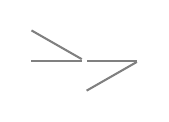
\begin{tikzpicture}[xscale=0.7, yscale=0.4]
        \pointedperson 34
        \person 14
        \person 15
        \person 24
        \person 23
        \linkpersons 3424
        \linkpersons 1524
        \linkpersons 1424
        \linkpersons 3423
    \end{tikzpicture}
}



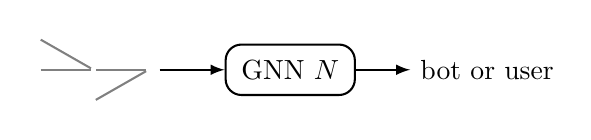
\begin{tikzpicture}
    \node (input) at (-2.5, 0)  {\examplesocialetwork};
    \node[draw, inner sep=2mm, rounded corners=2mm] (gnn) {GNN $N$};
    \node at (2.5, 0) (output) {bot or user};
    \draw (gnn) edge[-latex] (output);
    \draw (input) edge[-latex] (gnn);
\end{tikzpicture}
     %François: Sorry, updated the figure so that it takes less space + clearer I think
     \caption{Setting where a GNN $N$ is used to identify whether an account \faUser\ is a human or a bot in a fictitious social network.}
     \label{fig:gnn_social_network}
 \end{figure}

Unfortunately, like most neural network-based models, GNNs exhibit a black-box nature, making them particularly challenging to analyze. The ultimate goal in this context is \emph{formal reasoning}, which involves using sound and complete procedures to interpret the behavior of GNNs, and to certify or falsify specific safety properties of GNNs. Unfortunately, recent works such as (\citet{SalzerL23, benedikt2024decidability}) suggest that formal reasoning is practically intractable for highly expressive models like GNNs. Consequently, most of the research so far has focused on less rigorous types of reasoning, such as sound but incomplete or probabilistic procedures. For a comprehensive overview of non-formal verification procedures, see \citet{Gunnemann2022}.

% first we critize the current work
Several works build bridges between GNNs and logic (\cite{DBLP:conf/iclr/BarceloKM0RS20, benedikt2024decidability, ijcai2024}). However, they suffer essentially from two drawbacks. First, they consider idealized GNNs where weights and features are real numbers or arbitrary large integers. However, in practice, GNNs are \emph{quantized}, which means that numerical parameters and internal computations are constrained by a fixed representation size. For instance, the library \textsf{PyG} (\cite{Fey/Lenssen/2019}), based on PyTorch, designed to handle GNNs and other models, uses floating-point arithmetics of $32$ bits or $64$ bits. Furthermore, quantized GNNs are becoming increasingly important in tackling ever-growing model sizes by using very low numbers of bits to represent numerical model parameters (\cite{GholamiQuantized,ZhuLMH0LL023}). Second, previous works only consider truncated ReLU and other eventually constant activation functions (\cite{DBLP:conf/iclr/BarceloKM0RS20, ijcai2024}), or have limited results on GNNs utilizing the common ReLU activation (\cite{benedikt2024decidability}).

%then we present our contribution
The contributions of the paper are as follows.
\begin{itemize}
\item We introduce a logic \thelogic{} capturing a meaningful class of quantized (aggregate-combine) GNNs as well as linear input and output constraints on these GNNs (Section~\ref{sec:logic}).
\item We introduce a problem called linear-constrained validity problem (LVP) that enables to model properties like the ones in Example~\ref{fig:gnn_social_network}. We show how to solve LVP by reducing it to the satisfiability problem of \thelogic{} (Section~\ref{sec:gnntologic}).
\item We provide a proof system that enables to create graph counterexamples. A prototype of the proof system is implemented in Python. Noticeably, the proof system gives a PSPACE upper bound for a large class of GNNs, with any reasonable activation function (Section~\ref{sec:tableau}).
\item We also study the PSPACE lower bound and establish that LVP as well as satisfiability of \thelogic{} 
are indeed PSPACE-complete (Section~\ref{sec:lowerbound}).
\end{itemize}

%\begin{example}\label{ex:gnn_social_network_ctd}
%    For the safety property $A$ of Example~\ref{fig:gnn_social_network}, the input inequality would be $x_{\textit{msg\_count}} \geq 100$ where $x_{\textit{msg\_count}}$ is the feature corresponding to the number of messages sent by a user. The output property would look like $y \geq 0.6$, supposing that the GNN classifies a user as bot when its output is greater 
%    or equal than $0.6$. Now, finding a counterexample, meaning an input where the designated used has more or equal than $100$ sent messages and the GNN outputs a value less than $0.6$ indicates that the GNN does not satisfy property $A$.
%\end{example} 
%François thinks it is super boring to read a "technical example" in the introduction



% \todo{ms: do we have PSPACE for general sat? abstract states for bounded sat only}
% \todo{François does not understand what is "general sat". I suggest to keep it simple like it is.}
%\todo{maybe motivate more proof system, they are used to "certify"}

% \emph{Outline.} Section~\ref{sec:fundamentals} gives the preliminaries. Section~\ref{sec:logic} is dedicated to define syntax and semantics of \thelogic{}. In Section~\ref{sec:gnntologic}, we provide an efficient translation from LVP to \thelogic{} formulas, allowing to solve LVP using procedures to solve satisfiability of \thelogic{}. Afterwards, we show the PSPACE membership of the satisfiability problem of \thelogic{} via a tableau-like proof system in Section~\ref{sec:tableau}, and establish its PSPACE-hardness in Section~\ref{sec:lowerbound}. As it turns out, this implies the same bounds for LVP.  
% We close with a discussion of related work in Section~\ref{sec:relatedwork}, and  
% discuss perspectives in Section~\ref{sec:outlook}.

% \todo{I had another problem in mind. I mean there are persons doing agressive quantization to reduce the memory consumption. We could claim in the conclusion that our work could be used to verify these kind of agressive quantization.}

% %
% Quantized GNNs have lower memory consumption, faster inference, and can be deployed on resource-constrained devices.\todo[inline]{Say a bit more about the comsumption in Watts, real data, if not GNN, about DNN}



%\todo[inline]{We could expand by giving some interpretabilty (less bits to explain?) or ecological arguments (citation?)}





\section{Fundamentals}
\label{sec:fundamentals}

\newcommand{\setnumbers}{\mathbb K}
% 

\paragraph{Fixed-width Arithmetic} We consider different sets of numbers, denoted by $\setnumbers$, represented in binary using a fixed number of bits. Depending on the underlying (fixed-width) arithmetic, like fixed- or floating-point arithmetic, we denote the respective variants of operations like $+, \cdot, \div$ or relations like $\leq, \geq, =$ by $+_\setnumbers, \leq_\setnumbers, \dots$ and so on. For mathematically rigorous definitions of such arithmetics, see, for example,
\citet{Ercegovac2004,Goldberg91}.
% \citet{BaranowskiHLNR20,ConstantinidesD20}. 
To keep the notation uncluttered, we use $\setnumbers$ to refer to the
set of values as well as the underlying fixed-width arithmetic.
In general, we assume $\setnumbers$ contains $0$, $1$ and $-1$.
% Here are some examples\todo{or one example} for illustrative purposes.


% \begin{example}
% \label{example:signedint}
% In signed 32-bit integers, $\setnumbers$ is the set of numbers $\set{-2147483648, -2147483647, \dots, 2147483647}$.
% \end{example}

\begin{example}
\label{example:fixedpointarithmetic}
$16$-bit fixed-point arithmetic may be used in micro-controllers. For instance, $\setnumbers$ may be the set of numbers, of the form 
    $(-1)^s\frac{k}{10^{4}}$ with four decimal places precision,
    where $s \in \set{0, 1}$ is the sign, $k \in \{0, \dots, 2^{15}-1\}$.
\end{example}
% \todo{ms: why do we have denominator with base 10? shouldnt it be base 2?}
%François: because Nicolas needs that. I think it is also correct. We think there are no "standard" fixed-point arithmetic (contrary to IEEE754 for floating-point, so...)

%I agree, there is no "standard". The one we cited above Baranwoski et al. use base 2. but should be fine either way

\begin{example}
\label{example:floatingpointarithmetic}
In IEEE754 $32$-bit floating-point arithmetic, $\setnumbers$ exactly contains $0$, $-\infty$, $+\infty$ and numbers that are of the form 
    $(-1)^s 2^e(1+\frac{k}{2^{23}})$
    where $s \in \set{0, 1}$ is the sign, $e \in \set{-128, -125, \dots, 127}$, $k \in \set{0, \dots, 2^{23}-1}$. % The number $(1+\frac{k}{2^{23}})$ is called the \emph{significand}.
\end{example}

\paragraph{Graphs} We consider directed, vector-labelled graphs $G = (\nodes, \edges, \ell)$ where $\nodes$ is a finite set of nodes, or vertices,
$\edges$ is a set of directed edges and $\ell: V \rightarrow \mathbb{R}^m$.
We denote the class of all such graphs by $\graphs$.
We call a pair $(G,v)$ where $v$ is a node of $G$ a \emph{pointed graph}. We denote the class of all pointed graphs by $\pgraphs$.
If we restrict the classes $\graphs$ and $\pgraphs$ to vector labels with values from some fixed-width arithmetic $\setnumbers$, we denote this by $\graphs[\setnumbers]$ and $\pgraphs[\setnumbers]$.


\begin{figure}
    \centering
    	\begin{tikzpicture}[xscale=2,yscale=0.7]
		\draw[fill=white, opacity=0.7,rounded corners = 5mm, draw=none] (-2.5, 1.5) rectangle (0.6, -1.5);
		\node[inner sep=0mm, rounded corners=2mm] (0) at (-2, 0) {\labellednode{v}{1}{1}};
		\node[inner sep=0mm] (1) at (0, 1) {\labellednodeinv{v_1}{0.2}{1}};
		\node[inner sep=0mm] (2) at (0, -1) {\labellednodeinv{v_2}{1}{0.2}};
		\draw[->] (0) edge [bend left=10] (1);
		\draw[->] (0) edge [bend left=10] (2);
		\draw[->] (1) edge [bend left=10] (2);
		\draw[->] (2) edge [bend left=20] (0);
	\end{tikzpicture}
    \caption{Example of a vector-labelled graph.}
    \label{fig:graph}
\end{figure}
\begin{example}
    Figure~\ref{fig:graph} shows a vector-labelled graph with three nodes. Here $\ell : V \rightarrow \ensR^2$ and $\ell(v) = \begin{pmatrix}
        1\\1
    \end{pmatrix}$ for instance.
\end{example}



\paragraph{Graph Neural Networks} 
A \emph{Graph Neural Network (GNN)} $N$ is a tuple $(\layer_1, \dotsc, \layer_m, \layer_{\mathit{out}})$. Each layer $\layer_i$ computes 
$\layer_i(\boldsymbol{x}, M) = \comb_i(\boldsymbol{x}, \agg_i(M))$ where $\boldsymbol{x}$ is a real-valued vector, $M$ is a 
multiset of vectors, $\agg$ is called an \emph{aggregation function}, mapping a multiset of vectors onto a single vector, 
and $\comb$ is called a \emph{combination function}. Layer $\layer_{\mathit{out}}$ computes a function from vectors to vectors.
The GNN $N$ computes a function $\pgraphs \rightarrow \mathbb{R}^n$, where $n$ is the \emph{output dimension
of $N$}, in the following way. Let $(G, v)$ where $G=(V,E,\ell)$ be a pointed graph. 
First, $N$ computes a state $\boldsymbol{x}^m_u$
for all $u \in V$ in a layer-wise fashion by $\bs{x}^i_u = \comb_i(\boldsymbol{x}^{i-1}_u, \agg_i(\multset{\bs{x}^{i-1}_{u'} \mid (u,u') \in \edges}))$ 
and $\bs{x}^0_u = \ell(u)$. The overall output $N(G,v)$ is given by $\layer_{\mathit{out}}(\bs{x}^m_{v})$.
If we restrict the computation of $N$ to some fixed-width arithmetic, it computes a function 
$\pgraphs[\setnumbers] \rightarrow \setnumbers^n$ and we assume that all parameters of $N$ as well as internal
computations are carried out in $\setnumbers$. We call $N$ \emph{quantized (to $\setnumbers$)} in this case.


\begin{example}\label{ex:basic}
    Consider a GNN $N = (\layer_1, \layer_2, \layer_{out})$ with $\layer_i(\boldsymbol{x}, M) = \comb(\boldsymbol{x}, \agg(M))$
    where $\agg$ is the sum and with the same combination function $\comb: \mathbb{R}^{2\cdot2} \rightarrow \mathbb{R}^2$ in both layers where
    $\comb((x, x'),(\aggvar, \aggvar'))$ is given
    by
    \begin{displaymath}
    \left(\begin{matrix}
		\activationfunction(x + 2x' - 3\aggvar + 4\aggvar' + 5) \\
		\activationfunction(6x + 7x' + 8\aggvar - 9\aggvar' + 10) \\
	\end{matrix}\right)
 \end{displaymath}
 for some activation function $\activationfunction$, such as ReLU. The output layer $\layer_{out}$ 
 computes $\mathbb{R}^2 \rightarrow \mathbb{R}$ and is
 given by $\activationfunction(x_1 + x_2 - 2)$.
\end{example}


\section{Boolean Combinations Over Modal Expressions}
\label{sec:logic}

To reason about broad classes of GNNs and overcome the limitations of existing logical characterizations, we propose the logic $\thelogic{}$, which enables reasoning about general but quantized GNNs with arbitrary fixed-width arithmetic and activation functions. Existing characterizations, such as graded modal logic (\cite{DBLP:conf/iclr/BarceloKM0RS20}), modal logic on linear inequalities over counting (\cite{ijcai2024}), or fragments of Presburger logic (\cite{benedikt2024decidability}), typically relate to GNNs with eventually constant activation functions, like truncated ReLU $x \mapsto \max(0, \min(1,x))$. In contrast, $\thelogic{}$ extends beyond these constraints using the sole assumption of a quantized setting.

\subsection{Syntax}
Let $\featuresset$ be a finite set of features and $\setnumbers$ be some finite-width arithmetic. We consider a set of \emph{expressions} defined by the following Backus-Naur form:
%
$$\expression ::= c \mid x_i \mid \activationfunction (\expression) \mid \agreggationfunction (\expression) \mid %\agreggationfunctionglobalreadout(\expression) \mid
\expression + \expression \mid c\expression$$
%
where $c \in \setnumbers$, $i \in \featuresset$.
%
%
%
A \emph{formula} of the logic $\thelogic{}$ is then a Boolean formula where the atomic formulas are of the form $\expression \geq k$ for some $k \in \setnumbers$. 
When there is no ambiguity and to lighten the notation, we sometimes use more standard expressions, like $-x$ instead of $-1 \times x$, or $x \geq 4$ instead of $x + (-1) \times 4 \geq 0$, etc. We use $\expression = k$  as an abbreviation for
$(\expression \geq k) \land (-1 \times \expression + k \geq 0)$.
Formulas are represented as DAGs.
%
For example, in 
%$\expression \geq k \land -1\expression \geq -k$ 
$(\expression \geq k) \land (-1 \times \expression + k \geq 0)$
the expressions $\expression$ and $k$ are \emph{not} duplicated as shown in Figure~\ref{figure:dag}.
The symbol $\top$ denotes the tautology (any formula which is universally true, e.g., $x_1 - x_1 \geq 0$).
\begin{figure}
    \centering
    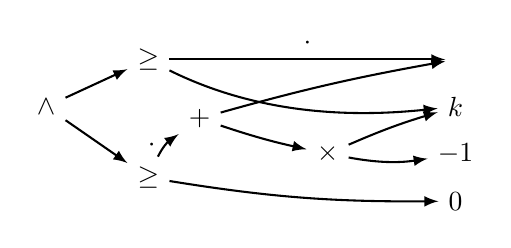
\begin{tikzpicture}[xscale=1.3,yscale=0.6]
        \node (E) at (1, 0) {$\expression$};
        \node (-1) at (1, -2) {$-1$};
        \node (k) at (1, -1) {$k$};
        \node (0) at (1, -3) {$0$};        
        \node (plus) at (-1.5, -1.25) {$+$};
        \node (times) at (-0.25, -2) {$\times$};
        \node (geq1) at (-2, 0) {$\geq$}; %geq at the top
        \node (geq2) at (-2, -2.5) {$\geq$}; %geq at the bottom
        \node (and) at (-3, -1) {$\land$};

        \draw[-latex] (geq1) edge[bend left=0] node [above] {$\cdot$} (E);
        \draw[-latex] (geq1) edge[bend right=30] (k);

        \draw[-latex] (geq2) edge[bend left=10] node [left] {$\cdot$} (plus);
        \draw[-latex] (geq2) edge[bend right=10] (0);

        \draw[-latex] (plus) edge[bend left=5] (E);
        \draw[-latex] (plus) edge[bend right=5] (times);
        \draw[-latex] (times) edge[bend left=5] (k);
        \draw[-latex] (times) edge[bend right=20] (-1);
          
         %\draw[-latex] (-2) -- (E);
           % \draw[-latex] (-) -- (k);
           %\draw[-latex] (-2) -- (E);
        \draw[-latex] (and) -- (geq1);
        \draw[-latex] (and) -- (geq2);
    \end{tikzpicture}
  
    \caption{DAG data structure for the formula 
    $(\expression \geq k) \land (-1 \times \expression + k \geq 0)$}
    \label{figure:dag}
\end{figure}




\subsection{Semantics}

\newcommand{\semone}[1]{[\![#1]\!]}
\newcommand{\sem}[2]{[\![#1]\!]_{#2}}

Recall that $\setnumbers$ is a finite set of numbers, equipped with an addition $+_\setnumbers$, multiplication $\times_\setnumbers$ operation, and comparison operations $\leq_\setnumbers$, $<_\setnumbers$.
We fix $\semone{\activationfunction}$ to be an activation function. For instance, $\semone{\activationfunction} = ReLU$, with $ReLU(x) = x$ if $x \geq_\setnumbers 0$ and $0$ otherwise. 
Formulas are evaluated over the class of pointed, labelled graphs $G = (\nodes, \edges, \ell)$ where $\ell : \nodes \rightarrow \setnumbers^I$, defined as follows.
The semantics $\sem{\expression} u$ of an expression $\expression$ with respect to a vertex $u\in V$ is inductively defined on $\expression$: 
\begin{center}
\begin{minipage}{40mm}
\begin{align*}
\sem {c} u & = c \\
    \sem {x_i} u & = \ell(u)_i \\
      \sem{\expression + \expression'} u & = \sem \expression u +_{\setnumbers} \sem {\expression'} u 
  \end{align*}
\end{minipage}
\hfill
\begin{minipage}{35mm}
\begin{align*}
  \sem{c \expression} u & = c \times_{\setnumbers} \sem{\expression} u \\
      \sem{\activationfunction (\expression)} u & = \semone{\activationfunction}(\sem \expression u)  \\
    \sem{\agreggationfunction (\expression)} u & = \Sigma_{v \mid u \edges v}\sem {\expression} v
    %\\
 %   \sem{\agreggationfunctionglobalreadout (\expression)} u & = \Sigma_{v \in \nodes}\sem {\expression} v
\end{align*}
\end{minipage}
\end{center}

%
The semantics $\sem{x_i}{u}$ is the value of $i$-th feature in vertex~$u$. 
Note that $\agreggationfunction(\expression)$
is motivated by the message-aggregation process in a GNN and is the `modal' part of $\thelogic{}$. Its semantics $\sem{\agreggationfunction(\expression)}{u}$ consists in summing up the values/semantics of $\expression$ in the successors $v$ of $u$.
We write $G, u \models \phi$ to say that the formula $\phi$ is true in the pointed graph $(G,u)$, and we say that $(G,u)$ is a \emph{model} of $\phi$. A formula $\phi$ is \emph{satisfiable} if it has a model. %there is a pointed graph $(G, u)$ such that $G, u \models \phi$.

\begin{example}
The formula $x_1 + \activationfunction(x_2) \geq 0$ is true in the pointed graphs $(G, u)$ where the sum of the first feature at $u$ plus the result of the application of the activation function on the second feature at $u$ is positive (i.e., $(\ell(u))_1 + \semone{\activationfunction}(\ell(u))_2 \geq_{\setnumbers} 0$).
The formula $\agreggationfunction(1) = 4$ is true in the pointed graphs $(G,u)$ with $u$ having exactly $4$ successors. The formula $\agreggationfunction(3) = 10$ is unsatisfiable.
\end{example}

\section{Enabling Formal Reasoning About GNNs Using $\thelogic{}$}
\label{sec:gnntologic}


Let us now formally define \emph{linear-constrained validity problem (LVP)} for GNNs.

\begin{definition}
%\todo[inline]{To be rigorous, we should have an explicit graph arity bound parameter: add in input ``given (max arity) $\arity \in \mathbb{N}$''; add in output ``where $v$ has max arity $\arity$''. Ignore? Introduce parameterized version later? Introduce here?}
%\todo{François: to be fully rigourous yes, but it makes noise a bit}
\emph{Linear-constrained validity problem (LVP)} for GNNs is defined as follows:
    \begin{itemize}
        \item given a GNN $N$ with input dimensionality $m$ and output dimensionality $n$
and two systems of linear inequalities $L_{\text{in}}$ over variables $x_1, \dotsc, x_m$ and 
$L_{\text{out}}$ over variables $y_1, \dotsc, y_n$,
\item decide whether $(N, L_{\text{in}}, L_{\text{out}})$ is \emph{valid}, that is all pointed-graphs $(G,v)$ where $v$ has $m$ features and $v$ satisfies system $L_{\text{in}}$ imply that $N(G,v)$ satisfies system~$L_{\text{out}}$. 
    \end{itemize}
\end{definition} 




\begin{example}
Recall the setting of Example~\ref{ex:gnn_social_network} where we considered the safety property, “Every account that spams $100$ messages or more per minute is identified as a bot by $N$.” 

This property is expressed by the LVP instance $(N, L_{\text{in}}, L_{\text{out}})$ with
$L_{\text{in}} := x_{\textit{msg\_count}} \geq 100$ and $L_{\text{out}} := y \geq 0.6$
where $x_{\textit{msg\_count}}$ is the feature corresponding to the number of messages sent by a user, and y is the output dimension of $N$ corresponding to its classification as a bot ($y \geq 0.6$) or a regular user ($y < 0.6$). Note that in this simple example $L_{\text{in}} $ and $L_{\text{out}}$ are systems consisting of a single inequality.
\end{example}

We show that LVP over quantized GNNs, where aggregation is given by summation, and combination functions and output functions are realized by classical feedforward neural networks (FNNs) using some kind of activation $\activationfunction$, is reducible to the satisfiability problem of \thelogic{}.
% \todo{see comment reviewer RqdA01; isn't the sentence still problematic? "and combination as linear combination?"}
%\todo{fixme? ... as linear combination/superposition?}
% To give an upper time-complexity bound for the corresponding translation, 

We denote the size of the GNN $N$ by $|N|$, with $|N| \in \mathcal{O}(|N_{\comb_1}| + \dotsb + |N_{\comb_m}| + |N_{\mathit{out}}|)$ where 
$m$ is the depth of $N$ and $|N_{\comb_i}|$ and 
$|N_{\mathit{out}}|$ are the sizes of the FNN used in $N$. The size of an FNN is simply the sum of the sizes of all its numerical parameters, namely weights and biases.


\begin{theorem}
\label{th:reduction}
    Let $I = (N, L_{\text{in}}, L_{\text{out}})$ be an LVP instance. There is a \thelogic{} formula $\varphi_I$ such that $I$ is valid 
    if and only if $\varphi_I$ is not satisfiable. Furthermore, $\varphi_I$ can be computed in polynomial time with respect to $|N| + |L_{\text{in}}| + |L_{\text{out}}|$.
\end{theorem}

\begin{proof}
    Let $I = (N, L_{\text{in}}, L_{\text{out}})$ be an LVP instance where the GNN $N$ has $l$ layers $\layer_i$, each having a combination function $\comb_i$
    represented by an FNN $N_{\comb_i}$ as well as aggregation function $\agg_i$ represented by the sum $\sum$ and output function represented by FNN $N_{\mathit{out}}$, $L_{\text{in}}$ consists of linear inequalities
    $\varphi_1, \dotsc, \varphi_{k_1}$ working over variables $x_1, \dotsc, x_{n_1}$ and $L_{\text{out}}$ consists of linear inequalities
    $\psi_1, \dotsc, \psi_{k_2}$ working over variables $y_1, \dotsc, y_{n_2}$.
    Formula $\varphi_I$ is the conjunction $\varphi_1 \land \dotsb \land \varphi_{k_1}\land \varphi_N \land (\neg\psi_1 \lor \dotsb \lor \neg\psi_{k_2})$ where $\varphi_N$ is constructed as follows. 
    Formula $\varphi_N$ is a conjunction
    $\expression_{N,y_1} - y_1 = 0 \land \dotsb \land \expression_{N,y_n} - y_{n_2} = 0$ where $\expression_{N, y_i}$ captures the computation of $N$ corresponding to its $i$-th
    output as follows.

    Consider layer $\layer_1$ and assume that $N_{\comb_1}$ has input dimension $2i_1$ and output dimension $o_1$. We define the sub-expression $\expression_{\layer_1, j}= \expression_{N_{\comb_1},j}(z_1, \dotsc, z_{i_1}, \agg(z_1), \dotsc, \agg(z_{i_1}))$ for $j \leq o_1$ where $\expression_{N_{\comb_1},j}$ is the straightforward unfolding of the function of $N_{\comb_1}$ corresponding to its $j$-th output using $c, c\expression, +$ and $\activationfunction(\expression)$ operators on the inputs 
    $z_1, \dotsc, \agg(z_{i_1})$. Next, consider the
    layers $\layer_h$ for $2 \leq h \leq l$. We assume that $N_{\comb_h}$ has input dimension $2o_{h-1}$ and output dimension $o_h$.
    We define the sub-expression $\expression_{\layer_h, j}$ equal to
    $\expression_{N_{\comb_h},j}(\expression_{\layer_{h-i},1}, \dotsc, \expression_{\layer_{h-1},o_{h-1}}, \agg(\expression_{\layer_{h-1},1}),$ $\dotsc$, $\agg(\expression_{\layer_{h-1},o_{h-1}}))$ for each $j \leq o_h$. Finally, we define $\expression_{N,x_j} = \expression_{N_{\mathit{out}, j}}(\expression_{\layer_m, 1}, \dotsc, \expression_{\layer_m, o_m})$ where $\expression_{N_{\mathit{out}, j}}$ is again the unfolding of the function of $N_{\mathit{out}}$ 
    corresponding to its $j$-th output.

    The correctness follows immediately from the construction above, as we simply unfold the computation of the GNN $N$ using operators available
    in \thelogic{}. The polynomial bound is due to the fact that we represent formulas as DAGs and, thus, avoiding any duplication of subformulas.
\end{proof}


\begin{example}
Consider the simple GNN $N$ of Example~\ref{ex:basic}.
The formula equivalent to $N$ in the sense of Theorem~\ref{th:reduction} is $\varphi_N := \activationfunction(\expression_{2}+ \expression_{2}') - y = 0$ with
\begin{align*}
    \expression_{i+1} & = \activationfunction(\expression_{i} + 2\expression_{i}' - 3\agg (\expression_{i}) + 4\agg (\expression_{i}') + 5), \\
    \expression_{i+1}' & = \activationfunction(6\expression_{i} + 7\expression_{i}' +8\agg( \expression_{i}) -9\agg (\expression_{i}') + 10),
\end{align*}
%
$\expression_0 = x$ and $\expression'_0 = x'$. Assuming that $L_{\text{in}} := x+x'\geq 0$ and
$L_{\text{out}} := y \geq 0.6$, the overall \thelogic{} formula would be
$\varphi_I := x+x'\geq 0 \land \varphi_N \land \lnot (y \geq 0.6)$.
\end{example}

In the sequel, we consider the quantized variant of LVP where numbers belong to $\setnumbers$. Furthermore, we bound the arity by $\arity$, that is the out-degree of each vertex in graphs $G$ is bounded by $\arity = k$, writing $(N, L_{\text{in}}, L_{\text{out}}, \delta = k)$.

\begin{remark}
The translation in Theorem~\ref{th:reduction} can be straightforwardly extended beyond the capabilities of LVP. For instance, we can generalize to instances of the form $(N, \varphi, \psi)$, where N is a GNN and $\varphi, \psi$ are \thelogic{} formulas.
\end{remark}



Note that if an LVP instance $I$ is not valid, then  $\varphi_I$ is satisfiable. A model of $\varphi_I$ offers a counterexample for $I$.



\section{Satisfiability of $\thelogic{}$ Formulas}
\label{sec:tableau}



In this section, we tackle the following satisfiability problem, in which $\arity$ is a bound on the arity of the pointed graph and $n$ is the number of bits to represent an element of $\setnumbers$. For instance, for $n = 32$, $\setnumbers$ could be %any of the Examples \ref{example:signedint}, \ref{example:fixedpointarithmetic}
\Cref{example:floatingpointarithmetic}. 
We write $\setnumbers_n$ to emphasize that numbers are encoded on $n$ bits. In the sequel, we fix a sequence $\setnumbers_0, \setnumbers_1, \setnumbers_2 \dots$ with the following reasonable polyspace assumption for each $\setnumbers_n$:
%For instance, To fix the ideas, we set $\setnumbers_n =  \set{-2^{n-1}, \dots, 2^{n-1}}$.
\begin{enumerate}
    % \item $\setnumbers_n$ is a set of numbers encoded with $n$ bits
    \item there is a uniform algorithm, taking $n$, $k_1$, $k_2$ and $k$ in $\setnumbers_n$ as an input and checking whether $k_1+k_2=k$ in poly-space in $n$ (same for checking whether $k_1=k_2$, $k\times k_1=k_2$)
    \item given $n$ written in unary, $k, k' \in \setnumbers_n$ written in binary, deciding whether
$\semone{\activationfunction}(k') = k$
can be performed in polynomial space in $n$. This assumption is weak and is true for a large class of activation functions $\semone{\activationfunction}$ (for instance $ReLU$, $truncatedReLU$ for fixed-point or floating-point arithmetics on $n$ bits).
\end{enumerate}


\begin{definition}[satisfiability problem]
The satisfiability problem of \thelogic{} is:
    \begin{itemize}
        \item input: an integer $n$ written in unary, an integer $\arity$ (or $\arity = +\infty$) in unary or in binary, a formula $\Phi$ in \thelogic{}
        \item question: does there exist a pointed graph of arity at most $\arity$ with features in a set $\setnumbers_n$ that satisfies $\phi$?
    \end{itemize}
\end{definition}

Note that $n$ is written unary is reasonable since $n$ is precisely of the same order of magnitude as the size of the representation of an element in $\setnumbers_n$, and we have to store the bits of numbers in $\setnumbers_n$ fully in memory anyway.

Bounding the arity $\delta$ is justified in applications such as chemistry.
%\todo{do we have applications in which we know in advance a bound on the arity? It would be nice to insert a sentence here}
Generally, it is sufficient to represent $\arity$ in unary since the bound is often small. For instance, a carbon atom has $4$ neighbors. Having $\arity$ in unary means also that we can keep all the successors/neighbors of a given vertex in memory at once.
A graph can be exponential in $\arity$; a tree may contain $\arity^{depth}$ nodes, making the search space exponential in the input size when the depth is unbounded. Using a binary representation for $\delta$ is also interesting since the search space is already exponential with a fixed depth. For instance, we could search for a pointed graph which is a tree of depth $1$ where the root has an exponential number of children.

\subsection{Tableau Method}


\begin{figure*}
\small
    \centering

%%%%% FIRST COLUMN
\begin{minipage}{0.45\linewidth}
     \begin{minipage}{0.45\textwidth}
 \begin{prooftree}
     \AxiomC{$(w~\phi \lor \psi)$}
     \rulelabel{\lor}
     \UnaryInfC{$(w~\phi) \mid (w~\psi)$}
 \end{prooftree}

 \begin{prooftree}
     \AxiomC{$(w~\lnot(\phi \lor \psi))$}
     \rulelabel{\lnot\lor}
     \UnaryInfC{$(w~\lnot \phi), (w~\lnot \psi)$}
 \end{prooftree}

 \begin{prooftree}
     \AxiomC{$(w~\phi \land \psi)$}
     \rulelabel{\land}
     \UnaryInfC{$(w~\phi), (w~\psi)$}
 \end{prooftree}
 \end{minipage}
 ~
 \begin{minipage}{0.45\textwidth}
 \begin{prooftree}
     \AxiomC{$(w~\lnot (\phi \land \psi))$}
     \rulelabel{\lnot\land}
     \UnaryInfC{$(w~\lnot \phi) \mid (w~\lnot \psi)$}
 \end{prooftree}

 \begin{prooftree}
     \AxiomC{$(w~\lnot \lnot \phi)$}
     \rulelabel{\lnot\lnot}
     \UnaryInfC{$(w~ \phi)$}
 \end{prooftree}
 \end{minipage}


\begin{prooftree}
    \AxiomC{$ (w~\lnot(\expression \geq k))$}
    \rulelabel{\lnot\geq}
    \UnaryInfC{$(w~\expression=k')$ for some $k' \in \setnumbers_n$ with $k' <_{\setnumbers_n} k$}
\end{prooftree}


%\begin{prooftree}
%	\AxiomC{$ (w~\lnot(\expression \geq k))$}
%	\rulelabel{\lnot \geq}
%	\UnaryInfC{$(w~\expression=-2^{n-1}) \mid (w~\expression=-2^{n-1}-1) \mid \dots \mid (w~\expression=k-1)$}
%\end{prooftree}


\begin{prooftree}
\AxiomC{$(w~\expression_1 + \expression_2 = k)$}
\rulelabel{+}
\UnaryInfC{\begin{minipage}{0.8\textwidth}
$(w~\expression_1 = k_1), (w~\expression_2 = k_2)$ for some $k_1, k_2 \in \setnumbers_n$,  with $k_1 +_{\setnumbers_n} k_2 = k$
\end{minipage}
}
\end{prooftree}

\begin{prooftree}
    \AxiomC{$(w~\phi)$ and no term $(w~arity=...)$}
\rulelabel{arity}
\UnaryInfC{$(w~arity=\delta')$ for some $\delta'\leq \delta$}
\end{prooftree}
\end{minipage}
%%%%% SECOND COLUMN
\begin{minipage}{0.45\linewidth}

\begin{prooftree}
\AxiomC{$(w~c = k)$ if $c \neq k$}
\rulelabel{clash_c}
\UnaryInfC{fail}
\end{prooftree}

\begin{prooftree}
\AxiomC{$(w~x_i = k), (w~x_i = k')$ if $k \neq k'$}
\rulelabel{clash_=}
\UnaryInfC{fail}
\end{prooftree}



\begin{prooftree}
\AxiomC{$(w~\activationfunction(\expression) = k)$}
\rulelabel{\activationfunction}
\UnaryInfC{$(w~\expression = k')$ for some $k' \in \setnumbers_n$ with $\semone{\activationfunction}(k') = k$}
\end{prooftree}

\begin{prooftree}
\AxiomC{$(w~\expression \geq k)$}
\rulelabel{\geq}
    \UnaryInfC{$(w~\expression=k')$ for some $k' \in \setnumbers_n$ with $k' \geq_{\setnumbers_n} k$}
\end{prooftree}

%\begin{prooftree}
%	\AxiomC{$(w~\expression \geq k)$}
%	\rulelabel{\geq}
%	\UnaryInfC{$(w~\expression = k) \mid (w~\expression = k+1) \mid \dots \mid (w~\expression = 2^{n-1}-1)$}
%\end{prooftree}

\begin{prooftree}
\AxiomC{$(w~c\expression = k)$}
\rulelabel{\times}
\UnaryInfC{$(w~\expression = k')$ for some $k' \in \setnumbers_n$ with $c \times_{\setnumbers_n} k' = k$}
\end{prooftree}


\begin{prooftree}
\AxiomC{$(w~\agg(\expression) = k)$}
\AxiomC{$(w~arity=\delta')$}
\rulelabel{\agg}
\BinaryInfC{
\begin{minipage}{0.8\textwidth}
$(w1~\expression = k_{1}), \dotsc, (w \arity'~\expression = k_{{\arity'}})$ for some $(k_u)_{u=1..\arity'}$, with $k_{1} +_{\setnumbers_n} 
 \dotsb +_{\setnumbers_n} k_{\arity'} = k$
\end{minipage}
}
\end{prooftree}

\end{minipage}

    \caption{Tableau rules for the satisfiability problem in \thelogic{} when $\delta$ is written in unary.
%    The rules for the Boolean connectives are standard, and are omitted for reasons of space.
}
    \label{figure:tableaurules}
\end{figure*}


We propose a tableau method (\cite{DBLP:books/el/RV01/Hahnle01,DBLP:books/daglib/0032750}) to reason in our logic, more specifically to check whether a formula $\Phi$ is satisfiable. For presentation purposes, we focus on the case where the arity bound $\arity$ is finite and given in unary. The cases where $\arity$ is written in binary or $\delta = +\infty$ are more involved, and are discussed in the Supplementary Material.

The idea of tableau methods is to construct a model satisfying an initial formula by propagating constraints and creating new vertices when needed.
We consider terms of the form $(w~\phi)$ where $w$ is a word (that intuitively denotes a vertex in the graph in construction) and $\phi$ is a formula. The intuitive meaning of $(w~\phi)$ is that $\phi$ should be true in the vertex $w$.

We start the tableau method with the following term $(\epsilon ~ \Phi)$, saying that $\Phi$ should be true in the initial vertex, denoted by the empty word $\epsilon$.
Figure~\ref{figure:tableaurules} shows our tableau rules. % The rules for the Boolean connectives are standard.

The rules for $(\lnot\geq), (\geq), (+), (\activationfunction), (\times)$ exploit the fact that the set $\setnumbers_n$ is finite. For instance, rule $(\geq)$ non-deterministically chooses a value for $\expression$ that is greater than $k$ in $\setnumbers_n$.
The rule $(+)$ on the term $(w~\expression_1+\expression_2=k)$ (whose meaning is that the value of $\expression_1+\expression_2$ should be equal to $k$) non-deterministically chooses values $k_1$ and $k_2$ for $\expression_1$ and $\expression_2$ respectively so that $k_1 + k_2 = k$.
The rule $(clash_c)$ stops the current execution when the constant $c$ is different from the value $k$ to which it is constrained to be equal. Similarly, the rule $(clash_=)$ clashes when the feature $x_i$ at the vertex denoted by $w$ is supposed to be equal to $k$ and $k'$ with $k\neq k'$. The rules $(\activationfunction)$ and $(\times)$ work similarly to the rule $(+)$ but for the activation function and for multiplication by a scalar. 
The rule $(arity)$ non-deterministically guesses the arity (number of successors) of the vertex specified by $w$.

The rule $(agg)$ is `modal' and creates new successors $w1, \dots, w\arity'$ where $w1$ is the word $w$ on which we concatenated the letter $1$, and so on. When the aggregation for the expression $\expression$ is supposed to be equal to $k$ and the arity is supposed to be $\delta'$, we create $\arity'$ successors and impose that the sum of the values of $\expression$ taken in these successors is equal to $k$ (to this aim, we non-deterministically choose values $k_1, \dots, k_{\arity'}$ for $\expression$ in these successors).

 The proposed tableau method is a non-deterministic procedure that applies as long as possible the rules given in Figure~\ref{figure:tableaurules} from the initial set $\set{(\epsilon~\Phi)}$.%, where $\epsilon$ is the empty word. 
 The method either fails or stops successfully if no more rules are applicable.

\subsection{Usage Example}


\label{sec:complete-example}
We assume that $\setnumbers$ is signed $32$-bit fixed-point numbers, with four decimal places precision, similar to Example~\ref{example:fixedpointarithmetic}.
%
The number $\frac{1}{125}$ is stored as (the binary encoding of the decimal number) $80$, $\frac{1}{1000}$ is stored as $10$, $0.9$ is stored as $9000$, $1000$ is stored as $10000000$, $250$ is stored as $2500000$, etc.
%
We also assume that the maximum arity $\arity$ is 5.

Elaborating on \Cref{ex:gnn_social_network}, consider the GNN $N = (\layer_1, \layer_{out})$ where $\layer_1 = (\agg_1, \comb_1)$, $\agg_1 = \sum$, $\comb_1((x_1), (\aggvar_1)) = \begin{pmatrix}
    ReLU(+\frac{1}{125}x_1 + 0\aggvar_1 + 0) \\
    Id(+0x_1 + \frac{1}{1000}\aggvar_1+ 0)
    \end{pmatrix}
    $.
So $N$ has only one layer, with input dimension $1$ (the value of $x_1$ that labels a node indicates the number of messages per minute sent by the individual), and output dimension~$2$. The output layer is the identity.
%
%
Consider also the LVP $I = (N, L_{\text{in}}, L_{\text{out}})$ where $L_{\text{in}} = x_1 \geq 100$ and $L_{\text{out}} = y_1 \geq 0.6$.
%




\paragraph{$\thelogic{}$ formula.}

As per \Cref{th:reduction} and its proof,
the LVP $I = (N, L_{\text{in}}, L_{\text{out}})$ is valid iff $\phi_I = \phi_{\text{in}} \land \phi_N \land \lnot \psi_{\text{out}}$ is not satisfiable, where:
\begin{itemize}
    \item $\phi_{\text{in}} := x_1 \geq 100$
    \item $\phi_N := ReLU(\frac{1}{125} x_1) - y_1 = 0 \land \frac{1}{1000}\agg(x_1) - y_2 = 0$
    \item $\psi_{\text{out}} := y_1 \geq 0.6$
\end{itemize}

\paragraph{Automated reasoning.}

We could show that
$(\agg(x_1) \geq 1000) 
\land \phi_N \land
\lnot (y_2 \geq 1.0)
$ is not satisfiable, establishing that $N$ comes with the guarantee of property $B$. Here we focus on property $A$.
%
If the pointed graph $(G,v)$ satisfies $L_{\text{in}}$, then $N(G,v)$ will satisfy $L_{\text{out}}$.
%
% Also, if $(G,v)$ has successors who send more than 1000 messages per minute in total, then $N(G,v)$ will satisfy $y_2 \geq 1.0$, indicating that $v$ may be part of a network of spammers.
%
% $(agg(x_1) \geq 1000) 
% \land 
% \phi_N
% \land
% \lnot (y_2 \geq 1.0)
% $ is unsatisfiable
%
%\todo[inline]{how could we make it formal...? Could imagine in the future having the $L_{in}$ constraint is expressed in the logic}
%
We could use the tableau method to automatically show that $\phi_I$ is not satisfiable and therefore that $I$ is valid. Unfortunately, a complete formal proof cannot be reasonably presented here or even done by hand.
%
Hence, to illustrate how the reasoning method can be used for the verification of quantized GNNs, we slightly modify the LVP $I$ with a different output constraint.

Let $I'$ be the LVP $(N, L_{\text{in}}, L'_{\text{out}}, \delta=5)$, where $N$ and $L_{\text{in}}$ are as before, and $L'_{\text{out}} := y_1 \geq 0.9$.
%
We are going to show that the new output constraint is not always satisfied. 
%
$I'$ is valid iff $\phi_{I'} := \phi_{\text{in}} \land \phi_N \land \lnot \psi'_{\text{out}}$ is not satisfiable, where:
\begin{itemize}
    % \item $\phi_{\text{in}} = x_1 \geq 100$
    % \item $\phi_N = \frac{1}{125} ReLU(x_1) - y_1 = 0 \land \frac{1}{1000}\agg(x_1) - y_2 = 0$
    \item $\psi'_{\text{out}} := y_1 \geq 0.9$
\end{itemize}

\newcommand{\ruledef}{\Delta}%\text{def}}

We employ our tableau method to prove that $\phi_{I'}$ is satisfiable and therefore that $I'$ is not valid.
%
We use $\checkmark$ to indicate that we have reached a term for which there are no rules to apply, except possibly $(clash_=)$. If in the end $(clash_=)$ does not apply, then we can read a model of $\phi_{I'}$ where the $\checkmark$s appear. 
We start the tableau method by applying the rule $(\land)$ and resolve inequalities with rules $(\geq)$ and $(\lnot \geq)$ (we write $(\ruledef)$ when we just use the definition of a formula):
\begin{prooftree}\small
\AxiomC{$(\epsilon ~ \phi_{\text{in}} \land \phi_N \land \lnot \psi'_{\text{out}})$}
\rulelabel{\land}
\UnaryInfC{$(\epsilon ~ \phi_{\text{in}}), (\epsilon ~ \phi_N), (\epsilon ~  \lnot \psi'_{\text{out}})$}
\end{prooftree}




\noindent
\begin{minipage}{0.15\textwidth}
\begin{prooftree}\scriptsize
\AxiomC{$(\epsilon ~ \phi_{\text{in}})$}
\rulelabel{\ruledef}
\UnaryInfC{$(\epsilon ~ x_1 {\geq} 100)$}
\rulelabel{\geq}
\UnaryInfC{$(\epsilon ~ x_1 {=} 100)$ $\checkmark$}
\end{prooftree}
\end{minipage}
%\hfill
     \begin{minipage}{0.15\textwidth}
     	\begin{prooftree}\scriptsize
     		\AxiomC{$(\epsilon ~ \phi_N)$}
     		\rulelabel{\ruledef}
     		\UnaryInfC{$(\epsilon ~ C_1 {\land} C_2)$}
     		\rulelabel{\land}
     		\UnaryInfC{$(\epsilon ~ C_1), (\epsilon ~ C_2)$}
     	\end{prooftree}
\end{minipage}
%\hfill
     \begin{minipage}{0.15\textwidth}
\begin{prooftree}\scriptsize
	\AxiomC{$(\epsilon ~ \lnot \psi'_{\text{out}})$}
	\rulelabel{\ruledef}
	\UnaryInfC{$(\epsilon ~ \lnot y_1{\geq} 0.9)$}
	\rulelabel{{\lnot} {\geq}}
	\UnaryInfC{$(\epsilon ~ y_1 {=} 0.8)$ %(non-det) 
		$\checkmark$}
\end{prooftree}
\end{minipage}

\noindent
where we write $C_1$ for the conjunct $ReLU(\frac{1}{125} x_1) - y_1 = 0$ and $C_2$ for the conjunct $\frac{1}{1000}\agg(x_1) - y_2 = 0$.


% \begin{prooftree}
% \AxiomC{$(\epsilon ~ \phi_N)$}
% \rulelabel{def}
% \UnaryInfC{$(\epsilon ~ \frac{1}{125} ReLU(x_1) + (-1) y_1 = 0 \land \frac{1}{1000}\agg(x_1) + (-1)y_2 = 0)$}
% \rulelabel{\land}
% \UnaryInfC{$(\epsilon ~ \frac{1}{125} ReLU(x_1) + (-1) y_1 = 0), (\epsilon ~ \frac{1}{1000}\agg(x_1) + (-1)y_2 = 0)$}
% \end{prooftree}



We handle the conjunct $C_1$ in $\phi_N$.
\begin{prooftree}\small
\AxiomC{$(\epsilon ~ ReLU(\frac{1}{125} x_1) + (-1) y_1 = 0)$}
\rulelabel{+}
\UnaryInfC{$
(\epsilon ~ ReLU(\frac{1}{125} x_1) = 0.8),
(\epsilon ~ (-1) y_1 = -0.8)
$ %(non-det)
}
\end{prooftree}


\begin{minipage}{0.25\textwidth}
	\begin{prooftree}\small
\AxiomC{$
(\epsilon ~ ReLU(\frac{1}{125} x_1) = 0.8)
$
}
\rulelabel{\alpha}
\UnaryInfC{$(\epsilon ~ \frac{1}{125} x_1 = 0.8)$} %(non-det)
% \end{prooftree}
% \begin{prooftree}\small
% \AxiomC{$(\epsilon ~ ReLU(x_1) = 100)$}
\rulelabel{\times}
\UnaryInfC{$(\epsilon ~ x_1 = 100)$ $\checkmark$} %(non-det)
\end{prooftree}
\end{minipage}
% Note that the $(\alpha)$ rule is non-deterministic in general, but only one value applies here.
%
\begin{minipage}{0.15\textwidth}
\begin{prooftree}\small
\AxiomC{$
(\epsilon ~ (-1) y_1 = -0.8)
$
}
\rulelabel{\times}
\UnaryInfC{$(\epsilon ~ y_1 = 0.8)$ $\checkmark$} %(non-det)
\end{prooftree}
\end{minipage}




Finally, we handle the conjunct $C_2$ in $\phi_N$.
\begin{prooftree}\small
\AxiomC{$(\epsilon ~ \frac{1}{1000}\agg(x_1) + (-1)y_2 = 0)$}
\rulelabel{+}
\UnaryInfC{$
(\epsilon ~ \frac{1}{1000}\agg(x_1) = 1),
(\epsilon ~ (-1)y_2 = -1)
$ %(non-det)
}
\end{prooftree}

\begin{minipage}{0.25\textwidth}
\begin{prooftree}\small
\AxiomC{$
(\epsilon ~ \frac{1}{1000}\agg(x_1) = 1)
$
}
\rulelabel{\times}
\UnaryInfC{$(\epsilon ~ \agg(x_1) = 1000)$ %(non-det)
}
% \end{prooftree}
% \begin{prooftree}\small
% \AxiomC{$
% (\epsilon ~ \frac{1}{1000}\agg(x_1) = 1)
% $
% }
\rulelabel{arity}
\UnaryInfC{$(\epsilon ~ arity = 4)$ $\checkmark$}
\end{prooftree}
\end{minipage}
\begin{minipage}{0.1\textwidth}
\begin{prooftree}\small
	\AxiomC{$
		(\epsilon ~ (-1)y_2 = -1)
		$
	}
	\rulelabel{\times}
	\UnaryInfC{$(\epsilon ~ y_2 = 1)$ %(non-det)
		$\checkmark$}
\end{prooftree}
\end{minipage}



\begin{prooftree}\small
\AxiomC{$(\epsilon ~ \agg(x_1) = 1000)$}
\AxiomC{$(\epsilon ~ arity = 4)$}
\rulelabel{\agg}
\BinaryInfC{$(1 ~ x_1 = 250), \dotsc, (4 ~ x_1 = 250)$ %(non-det) 
$\checkmark$}
\end{prooftree}
% That is, five (which is the maximum arity $\arity$) worlds $w_1, \dotsc w_5$ where $x_1 = 200$ are witnesses of the formula $\agg(x_1) = 1000$.



\paragraph{Obtaining a model.}
We obtain a counterexample $(G,v)$ for the formula $\phi_{I'}$, with the node $v$ labeled $(x_1) = (100)$, which has $4$ successors, all labeled $(x_1) = (250)$. 
%
So, by \Cref{th:reduction}, $I'$ is not valid.
%
Indeed, $G,v$ satisfies $L_{in}$. But $N(G,v)$ is $(y_1, y_2) = (0.8, 1)$ which does not satisfy $L'_{out}$.

This illustrates how the proof system serves to verify the properties of quantized GNN, but also to exhibit counterexamples when they exist.








%\todo{to do with fix-point arithmetics}
%\begin{center}
%    \begin{algo}
%        \begin{algoblocprocedure}
%            {$check(E, y)$}%
%
%\begin{algomatch}
 %   {$\expression$}
    
%\algocase $x_i$: 
 %   
%\end{algomatch}

            
 %       \end{algoblocprocedure}
 %   \end{algo}
%\end{center}

%The interesting reader may have a look to 
A prototype implementation of the proof system is presented in Section~\ref{appendix-section-implementation} of the Supplementary Material.


\subsection{Upper Bound}

\begin{theorem}
\label{th:satlogPSPACE}
The satisfiability problem of $\thelogic$ is in PSPACE, whether $\delta$ is given in unary, binary or is infinite.
\end{theorem}

\begin{proof}
The proof is given for $\delta$ in unary.  For the proof when~$\delta$ in binary or infinite, we can adapt the proof system, see Supplementary Material, Section~\ref{sec:proofs-arity-binary-or-unbounded}.
   We have to prove that $\Phi$ is satisfiable iff there is an accepting execution of the tableau method.
    
    The \fbox{$\Rightarrow$} direction is proven by taking a pointed graph $G, v$ satisfying $\Phi$ and making the non-deterministic choices by letting oneself be guided by the evaluation of formulas in $G$. 
    To do that, we start the execution of the tableau method with $(\epsilon~~ \phi)$ and we set $f(\epsilon) = v$. We then show that we can always continue the execution maintaining the invariant:
    the partial mapping $f$ from the labels in the tableau to $V$ is such that if $(w~\phi)$ appears in the tableau then $G, f(w) \models \phi$; and if $(w~arity=\delta')$ appears then $f(w)$ is of arity $\delta'$.
    
    More precisely, we make the non-deterministic choices so that we can build a partial mapping $f$ from the labels in the tableau to $V$, starting from $f(\epsilon) = v$ so that if $(w~\phi)$ appears in the tableau then $G, f(w) \models \phi$; and if $(w~arity=\delta')$ appears then $f(w)$ is of arity $\delta'$. 
    
    Let us explain the principle with the $(agg)$ rule. Suppose $(w~\agg(\expression) = k)$ and $(w~arity=\delta')$ appears in the tableau. By the invariant, it means that $G, f(w) \models \agg(\expression) = k$ and that $f(w)$ is of arity $\delta'$. But then $f(w)$ has $\delta'$ successors: $u_1, \dots, u_{\delta'}$. As $G, f(w) \models \agg(\expression) = k$, there exists $k_{1}, \dots, k_{{\arity'}}$ with $k_{1} +_{\setnumbers_n} 
 \dotsb +_{\setnumbers_n} k_{\arity'} = k$ with $G, u_i \models \expression = k_i$ for all $i=1..\delta'$.
We then set $f(w1) := u_1, \dots, f(w\delta') = u_{\delta'}$. We also apply the rule $(agg)$ by choosing $(w1~\expression = k_{1}), \dotsc, (w \arity'~\expression = k_{{\arity'}})$. The invariant remains true.

By the invariant, the premises of rules $(clash_c)$ or $(clash_=)$ are never in the tableau. For instance, if some $(w~~c=k)$ with $c \neq k$ appears, we would $G, w \models c=k$ which is a contradiction.


    
    The \fbox{$\Leftarrow$} direction is proven by constructing a pointed graph $G, v$ from the choices made in the accepting execution. The graph $G = (V, E)$ is defined with $V$ the set of labels $w$ and $E$ is the set of edges of the form $(w, wu)$ with $w$ a label and $u \in \set{1, \dots, \delta'}$ with $(w~~arity=\delta')$ appearing in the tableau. The label is $\ell(w) = (v_1, \dots, v_m)$ with $v_i$ such that $(w~x_i=v_i)$ appears in the tableau, or $v_i$ can be any number in $\setnumbers_n$ if no term $(w~x_i=...)$ appears.

    We then prove that $G, \epsilon \models \phi$. To do that, we prove that if $(w~~\psi)$ appears in the final tableau, then $G, w \models \psi$ by induction on $\psi$.
    %
    We show it for $\psi =: \agg(\expression) = k$.
    Suppose that $(w~~\agg(\expression) = k)$ appears in the final tableau. Then it means that the rule $(\agg)$ has been applied on it. So $(w1~\expression = k_{1}), \dotsc, (w \arity'~\expression = k_{{\arity'}})$ for some $(k_u)_{u=1..\arity'}$, with $k_{1} +_{\setnumbers_n} 
 \dotsb +_{\setnumbers_n} k_{\arity'} = k$ appear in the final tableau. By induction, it means that $G, wi \models \expression = k_{i}$. So $G, w \models \agg(\expression) = k$.
Finally, as $(\epsilon~~\phi)$ is in the tableau, the induction hypothesis gives $G, \epsilon \models \phi$.


It can be implemented in poly-space, in the same spirit as the tableau method for modal logic K (\cite{DBLP:journals/ai/HalpernM92}). The idea is to backtrack on rules $(\agg)$: first we try to add all the $(w1~\expression = k_{1})$ for all applications of $(\agg)$, then try to add the $(w2~\expression = k_{2})$ and so on. The algorithm is then a depth-first-search on the tree relying on the labels $w$ (see \Cref{figure:searchtree}). We conclude by Savitch's theorem (\cite{DBLP:journals/jcss/Savitch70}) to obtain a deterministic algorithm.
\end{proof}



\begin{figure}
	\centering
		\small
	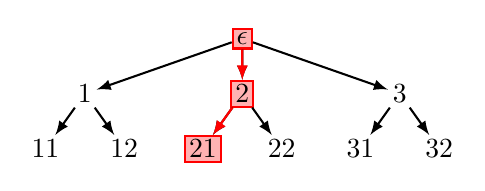
\begin{tikzpicture}[
		every node/.style = {inner sep=0.5mm},
		level distance = 7mm,
		edge from parent/.style = {draw, -latex},
		sibling distance = 2cm, % Set a default sibling distance
		level 2/.style = {sibling distance=1cm}, % Custom sibling distance for level 2
		]
		
		\node[fill=red!30, draw=red] (r) {$\epsilon$}
		child {node {1}
			child {node {11}}
			child {node {12}}
		}
		child {node[fill=red!30, draw=red] (2) {2}
			child {node[fill=red!30, draw=red] (21) {21}}
			child {node {22}}
		}
		child {node {3}
			child {node {31}}
			child {node {32}}
		};
	
	\path[draw=red, thick, -latex] (r) -- (2);
	\path[draw=red, thick, -latex] (2) -- (21);
		
	\end{tikzpicture}
	\caption{Depth-first search tree where each node contains terms of the form $(w~~...)$ for a given word $w$ among $\epsilon, 1, 2, 3, 11, 12, 21, 22, 31, 32$. Only a single branch is in memory.
 }
  \label{figure:searchtree}
 
\end{figure}





Now, Theorem~\ref{th:reduction} and \ref{th:satlogPSPACE} imply an upper bound for LVP. 
\begin{corollary}
\label{cor:LVPPSPACE}
    LVP is in PSPACE.
\end{corollary}


Note that when $\arity$ is in unary, the satisfiability problem is in NP when the number of nested $\agg$ operators in the input formula is bounded by a fixed integer $i$. Indeed, the certificate is a pointed labelled tree of depth $i$ of arity at most $\delta$ (it contains $O(\delta^i)$ vertices). In consequence, LVP when we bound the number of layers by~$i$ is in coNP.



\section{Lower Bounds}

%\subsection{Restricted Cases}

\label{sec:lowerbound}
\newcommand{\setofvaluesforPSPACEhardaritytwo}{\set{ 0, 1, 2}}
\newcommand{\setofvaluesforPSPACEhard}{\set{-2, -1, 0, 1, 2, 3}}

\newcommand{\casezerotwoatwo}{$\text{Case}_{\set{0,1,2}, \delta=2}$}
\newcommand{\caseminustwothree}{$\text{Case}_{\set{-2..3}, satu}$}

If not said otherwise, we suppose now the activation function is truncated ReLU; it corresponds to the settings in many works (\cite{DBLP:conf/iclr/BarceloKM0RS20,ijcai2024, benedikt2024decidability}). Furthermore, to obtain stronger PSPACE lower bound results, we will consider two restrictions:
\begin{itemize}
    \item \casezerotwoatwo: either $\setnumbers$ contains $0$, $1$, $2$ %$\setofvaluesforPSPACEhardaritytwo$ 
    and the arity is bounded by $\arity{=}2$;
    \item \caseminustwothree: or $\setnumbers$ includes $\setofvaluesforPSPACEhard$ and moreover, $\setnumbers$ saturates in the following sense: for all integers $x$, $x \geq 3$ implies $x_\setnumbers \geq_\setnumbers 3_\setnumbers$. In particular, it means that we have no modulo behavior in $\setnumbers$ (e.g., $\setnumbers = \mathbb Z_{10}$ would not saturate since despite $10 \geq 9$ as integers, we would not have $0 = 10 \geq_\setnumbers 9$ modulo $10$).
\end{itemize}
In both cases, $n=3$ bits are enough to represent the numbers.
Our lower bound results rely on \emph{graded modal logic} which extends modal logic with constructions $\gmlbox k \phi$ whose truth conditions is:
    $G, v \models \gmlbox k \phi$  iff there are at least $k$ successors $u$ of $v$ such that $G, u \models \phi$.
We call $\text{GML}_K$ the syntactic fragment 
%of GML 
where occurrences of $\gmlbox k$ are such that $k \leq K$.




\begin{lemma}
The satisfiability of $\fragmentGMLmodallogic$ on graphs of arity at most $2$, and the satisfiability of $\fragmentGML$ is PSPACE-hard.
\label{lemma:GMLonegrapharitytwo}
\label{lemma:GMLthree}
\end{lemma}

% \begin{lemma}

% \end{lemma}



%\subsection{PSPACE-hardness}
%We refer to these assumptions as the \emph{restricted cases}.
 
 
 %The PSPACE-hardness already holds because it embeds modal logic over complete binary trees.
%The values 0, 1, 2 encode that a formula $\phi$ is respectively false in all successors, true in exactly one successor, true in both successors.

\begin{theorem}
    LVP is PSPACE-complete. PSPACE-hardness holds already for \casezerotwoatwo\ or \caseminustwothree.
    \label{theorem:LVPPSPACEcomplete}
\end{theorem}

\begin{proof}
PSPACE-membership is stated in Corollary~\ref{cor:LVPPSPACE}. The lower bound relies on the poly-time transformation $\tau$ of a GML-formula $\phi$ into an equivalent GNN $\aGNN = \tau(\phi)$ in the sense that $\aGNN(G, v)$ satisfies $x_1 \geq 1$, given in \citet [proof of Proposition~4.1]{DBLP:conf/iclr/BarceloKM0RS20}. More specifically, we carefully analyse the GNN $N$ when the formula $\phi$ is in $\text{GML}_K$.

In $N$, the activation function is truncated ReLU. 
The layers in $\tau(\phi)$ are all the same. The matrices $C$ contain coefficients $-1$, $0$, $1$ and all coefficients on a column are $0$ except two at most.
The matrices $A$ only contain $0$ and $1$. On each column of $A$, all coefficients are $0$ except one which may be~$1$.
Coefficients in the biases $b$ are in $\set{ -K{+}1, -K{+}2, \dots, 1}$. 


Propositional variables in $\phi$ are among $p_1, \dots, p_J$, 
$\aGNN(G, v)$ starts with the initial state 
$(\bs{x}^0_u)_j = 1$, if $j \in \set{1, \dots, J}$ and $p_j$ holds in $u$, and $(\bs{x}^0_u)_j = 0$ otherwise.
% $(\bs{x}^0_u)_j = \begin{cases}
%     1 \text{ if $j \in \set{1, \dots, J}$ and $p_j$ holds in $u$} \\
%     0 \text{ otherwise.}
% \end{cases}$
%
 As the activation function is truncated ReLU, all vectors $\bs{x}^i_u$ are $0$--$1$-vectors.
 
 
Given the coefficients in the matrices, intermediate values are all integers.% The numbers in the computation of $\aGNN(G, v)$ stay in $\setofvaluesforPSPACEhard$. 
%
We end the proof of our Theorem~\ref{theorem:LVPPSPACEcomplete} by stating the reductions and arguing that the computation is \emph{safe} when done in~$\setnumbers$, meaning that there is no overflow and that the computation in~$\setnumbers$ and in 
%the set of integers 
$\mathbb{Z}$ yields the same result.
    
\newcommand{\LVPdual}{\ensuremath{\compl{\text{LVP}}}\xspace}

\paragraph{Proof for \casezerotwoatwo} 
We reduce the satisfiability of $\fragmentGMLmodallogic$ on graphs of arity at most $2$ which is PSPACE-hard (\Cref{lemma:GMLonegrapharitytwo}) into the dual problem \LVPdual of LVP with $\delta {=} 2$: from $\phi$ a $\fragmentGMLmodallogic$-formula, we compute the \LVPdual-instance $(\tau(\phi), \top, y_1 \leq 0, \arity=2)$, and $\phi$ is satisfiable on graphs of arity $2$ iff $(\tau(\phi), \top, y_1 \leq 0, \arity=2)$ is a negative instance of LVP. \LVPdual is PSPACE-hard, so is LVP. The computation is safe because there are at most two successors, so we never exceed $2$ in a computation in $\setnumbers$.

\paragraph{Proof for \caseminustwothree} 
 We reduce the satisfiability of $\fragmentGML$ which is PSPACE-hard (\Cref{lemma:GMLthree}) into \LVPdual: given $\phi$ a $\fragmentGML$-formula, we compute the \LVPdual-instance $(\tau(\phi), \top, y_1 \leq 0, \delta{=}{+\infty})$.
%\todo{not sure about the notation of this instance. $\delta{=}+\infty$ out of instance? And it should be $(\tau(\phi), x_1 - x_1 \leq 0, y_1 \leq 0)$? Same afterwards.}
%\todo{$\top$ has now been introduced in the syntax section. $\delta$ is given in the input, see end of section 4}
%\todo{But the parameters of LVM are not formulas :-). I've introduce the notation explicitly, which does not look so pretty}
We have that $\phi$ is $\fragmentGML$-satisfiable iff there exists $G, v$ s.t.\ $G, v \models \phi$ iff $(\tau(\phi), \top, y_1 \leq 0, \delta{=}{+\infty})$ is a negative instance of LVP. 
The computation is safe because, even if there are an arbitrary large number $x$ of successors, if $x \geq 3$, we also have $x_{\setnumbers} \geq_{\setnumbers}  3_{\setnumbers}$ because $\setnumbers$ saturates.
\end{proof}



\begin{corollary}
\label{corollary-satthelogicPSPACEc}
The satisfiability problem of \thelogic{} is PSPACE-complete, and already PSPACE-hard for \casezerotwoatwo\ or \caseminustwothree, and also when the activation function is ReLU.
\end{corollary}


% \section{Implementation}
% \label{sec:implementation}

% \todo[inline]{Marco?}



\section{Related Work}
\label{sec:relatedwork}
Starting with Graded Modal Logic  (\cite{DBLP:journals/ndjfl/Fine72}),
there are numerous logics that capture modal aspects of graphs and express arithmetic constraints, (\cite{
DBLP:journals/japll/DemriL10,
% DBLP:conf/frocos/Baader17,
DBLP:conf/frocos/BaaderB19,
% DBLP:conf/ekaw/GallianiRKPT20,
DBLP:conf/fsttcs/BednarczykOPT21,
DBLP:conf/kr/GallianiKT23,
DBLP:journals/bsl/BenthemI23}). 
% At the difference of $\thelogic{}$ which is parameterized with a fixed-width arithmetic, all existing works operate over all integers or rational numbers.

Previous research has already established several correspondences between logic and GNNs. For instance, \citet{DBLP:conf/iclr/BarceloKM0RS20} explored the relationship between graded modal logic and GNNs, while \citet{ijcai2024} examined modal logic on over linear inequalities with counting and its connection to GNNs. Additionally, \citet{benedikt2024decidability} investigated fragments of Presburger logic in the context of GNNs. However, these existing works focus on GNNs with specific activation functions and do not consider the broader class of quantized GNNs. In particular, decidability in PSPACE has been established only for cases where the activation function is either a truncated ReLU (\cite{ijcai2024}) or eventually constant functions (\cite{benedikt2024decidability}). 
More loosely related, is the work of \citet{Grohe23}, which establishes that the graph queries computable by a polynomial-size, bounded-depth family of GNNs are precisely those definable in the guarded fragment  \text{GFO+C}  of first-order logic with counting and built-in relations. This finding situates GNNs within the circuit complexity class  $\text{TC}^0$.

%\citet{HenzingerLZ21} also addresses the verification of quantized neural networks, in particular feedforward neural networks. The authors claim to establish a PSPACE-hardness result. However, the precise setting of 
%representation sizes they assume is not explicitly clarified and is likely to be logarithmic, which presumably causes the hardness result. In other cases, such as when using a unary representation as considered in 
%this paper, the problem is presumably in NP. But, a rigorous proof or detailed analysis of the sometimes vague arguments used in \citet{HenzingerLZ21} is left as future work. 
%Thank you! François likes BUT "rigorous proof" etc. is a bit attacking their paper

\citet{HenzingerLZ21} also addresses the verification of quantized neural networks, but in contrast to this paper they focus on FNN. The authors establish a PSPACE-hardness result, relying on a binary representation of the number of bits. In contrast, if the number of bits were unary, their problem is presumably in NP (using a guess and check argument, relying on similar arguments as used by \cite{SalzerL21}).
%Marco : put your paper in XXXXXXXXX where 
%However, their lower bound is so because the number of bits seems to be written in binary and not in unary as our paper. Their PSPACE-hardnesin their setting, the precise setting of 
% This highlights the greater complexity of verifying GNNs compared to FNNs.
% This underscores that verifying GNNs is fundamentally more complex than verifying `standard’ neural networks. and necessitates specialized techniques.

There are other aggregation functions, like weighted sums in graph attention networks \cite{DBLP:conf/iclr/VelickovicCCRLB18}, maximum in Max-GNNs \cite{DBLP:conf/kr/CucalaG24}, or average. \thelogic{} and the tableau method can be adapted to capture these aggregation functions, too (see Supplementary Material, Section~\ref{appendix-section-aggregation}). 
% \todo{maybe say explicity that our work is not a consequence of their work}

On the practical side, \citet{DBLP:conf/aaai/000200DWZB24} presents a solution to the verification of quantized FNNs using heuristic search, and outperforming the approach of \citet{10.1145/3551349.3556916} based purely on integer linear programming.

\section{Conclusion and Perspectives}
\label{sec:outlook}

We introduced a method for explicitly verifying and reasoning about properties of a practical class of quantized Graph Neural Networks. 
% with arbitrary activation functions. 
It allows us to establish new foundational results about the computational complexity of GNNs' tasks.

We proposed a tableau method for reasoning about quantized GNNs using the newly introduced logic \thelogic{}. As the domain for numbers is finite, we are able to work out our details using a parametrized class of quantized GNNs, allowing us to consider various activation functions.
We showed that for such classes of GNNs using FNNs in their internal parts, we can answer basic formal reasoning questions using a reduction to the satisfiability problem of \thelogic{}.
We showed that satisfiability of  \thelogic{}
%assuming a fixed bound on the arity of satisfying (pointed) graphs 
is solvable in PSPACE. 

%\todo{explain that the case undirected can be also handle (cf. inspired from tableau method for KB + cite instead of K}

This work is a first step to further develop concrete methods for reasoning about quantized GNNs and other neural network models. Now, it will be interesting to implement our approach on  a broader scale in order to tackle tasks such as certifying (adversarial) robustness properties (\cite{Gunnemann2022}) or giving formal explanations (\cite{0001I22_formalxai}) for certain GNN behaviours.

\section*{Ethical Statement}
There are no ethical concerns.